\documentclass[12pt,a4]{report}
\usepackage{textcomp}
\usepackage{fancyhdr}
\usepackage{graphicx}
\usepackage{titletoc,tocloft}
\usepackage{enumitem}
\usepackage{amsmath,amssymb}
\evensidemargin 0.5in
\oddsidemargin 0.0in
\topmargin 0.5in
\textwidth 6.5in
\headheight 0.3in
\headsep 0in
\usepackage[]{hyperref}
\usepackage{tikz}
\usetikzlibrary{arrows,shapes,snakes,automata,backgrounds,petri}
\usepackage{tabularx}
\usepackage{pgfgantt}
\usepackage[margin=1in]{geometry}
\usepackage{lscape}
\usepackage{array}
\usepackage{longtable}
\usepackage{multirow}
\usepackage[titletoc]{appendix}
\renewcommand{\bibname}{References}
\setcounter{secnumdepth}{5}
\usepackage{float}
\usepackage{subcaption}
\usepackage{multirow}
\usepackage{longtable}
\usepackage{geometry}
\geometry{margin=1in}
\usepackage{caption}
\usepackage[ruled,vlined]{algorithm2e}
\newcommand{\cellpadding}{\renewcommand{\arraystretch}{1.2}}
\newcommand{\headerpadding}{\renewcommand{\arraystretch}{1.5}}
\newcolumntype{P}[1]{>{\raggedright\arraybackslash}p{#1}}
\textheight 8.5in
\newcommand{\pa}{\hspace{3ex}}
\newcommand{\be}{\begin{equation}}
\newcommand{\ee}{\end{equation}}
\newcommand{\fs}{\hspace{2ex}}
\newcommand{\no}{\noindent}
\newcommand{\hs}{\hspace{1ex}}
\newtheorem{myth}{Theorem}
\newtheorem{prop}{Proposition}
\newtheorem{cor}{Corollary}
\newtheorem{defn}{Definition}
\newcommand{\vs}{\vspace{0.2in}}
\newcommand{\im}{{\lfloor m \rfloor}}
\newtheorem{obs}{Observation}
\newtheorem{lemma}{Lemma}
\newcommand{\vf}{{\vspace{0.50in}}}
\newcommand{\ms}{\;}
\newcommand{\createGanttChart}{%
    \begin{table}[htbp]
    \centering
    \begingroup
    \renewcommand\sfdefault{phv}
    \renewcommand\mddefault{mc}
    \renewcommand\bfdefault{bc}
    \sffamily
    \begin{ganttchart}[
        canvas/.append style={fill=none, draw=black!5, line width=.75pt},
        hgrid style/.style={draw=black!5, line width=.75pt},
        vgrid={*1{draw=black!5, line width=.75pt}},
        title/.style={draw=none, fill=none},
        title label font=\bfseries\footnotesize,
        title label node/.append style={below=7pt},
        include title in canvas=false,
        bar label font=\mdseries\small\color{black!70},
        bar label node/.append style={left=2cm},
        bar/.append style={draw=none, fill=black!63},
        bar incomplete/.append style={fill=blue!40},
        bar progress label font=\mdseries\footnotesize\color{black!70},
        group left shift=0,
        group right shift=0,
        group height=.5,
        group peaks tip position=0,
        group label node/.append style={left=.6cm},
        group progress label font=\bfseries\small,
        x unit=0.7cm,
        title label node/.append style={xshift=0.1cm}
    ]{1}{12}
      \gantttitle[
        title label node/.append style={below left=7pt and -3pt}
      ]{2026}{12} \\
      \gantttitlelist[
        title label node/.append style={below left=7pt and -3pt}
      ]{{"Jan"}, {"Feb"}, {"Mar"}, {"Apr"}, {"May"}, {"Jun"}, {"Jul"}, {"Aug"}, {"Sep"}, {"Oct"}, {"Nov"}, {"Dec"}}{1} \\
      \ganttgroup{Project Timeline}{1}{12} \\
      \ganttbar[name=planning]{\textbf{1.} Requirements \& Literature Review}{1}{2} \\
      \ganttbar[name=research]{\textbf{2.} Dataset Collection \& Preprocessing}{3}{4} \\
      \ganttbar[name=dataset]{\textbf{3.} CNN/ViT Model Development}{5}{6} \\
      \ganttbar[name=prototype]{\textbf{4.} LLM + RAG Pipeline Integration}{7}{8} \\
      \ganttbar[name=testing]{\textbf{5.} Frontend \& Backend Development}{9}{10} \\
      \ganttbar[name=implementation]{\textbf{6.} Testing, Validation \& Deployment}{11}{12}\\
      \ganttbar[name=documentation]{\textbf{7.} Documentation}{10}{12}
    \end{ganttchart}
    \endgroup
    \caption{Project Timeline}
    \label{gantt:project-timeline}
    \end{table}
}
\input{psfig.sty}

\begin{document}
\pagebreak
\pagenumbering{gobble}
\vspace*{\fill}
\begin{center}


 {\large A PROJECT BASED SEMINAR REPORT}\\
\vspace{0.5cm}
on\\
\vspace{0.5cm}

{\bfseries \fontsize{16}{20}\selectfont
Multi-Model AI-Based Personalized Skincare\\
Recommendation System\\
}
 
 \\ \vspace*{2\baselineskip}}
{\bfseries \fontsize{13}{12} \selectfont{for Hormonal Skin Conditions}  \\ \vspace*{2\baselineskip}}
{\fontsize{12}{12} \selectfont Submitted towards the
 \\Partial Fulfilment of the Requirements of} \\
\vspace{0.5cm}
{\bfseries \fontsize{14}{12} \selectfont Bachelor of Technology in \\Artificial Intelligence and Data Science\\
\vspace*{1\baselineskip}}
 By \\
{\large \begin{center}
\begin{tabular}{l l}
Shaikh Mohammed Ateeb        & Seat No: T231311117 \\
\end{tabular}
\end{center}}
Under the guidance of \\
\vspace{0.5cm}
{\bfseries \large Prof. Pranali Shinde} \\ \vspace{0.5cm}

\begin{figure}[!h]
\centering
  
\includegraphics[width=1.5in]{Logo.png}
\end{figure}

{\small Department of Artificial Intelligence and Data Science}\\
K. K. WAGH EDUCATION SOCIETY\\
K. K. WAGH INSTITUTE OF ENGINEERING EDUCATION AND RESEARCH\\
Hirabai Haridas Vidyanagari, Amrutdham, Panchavati, Nashik, Maharashtra 422003 \\
(An Autonomous Institute affiliated to Savitribai Phule Pune University)\\
A. Y. 2025-2026 Sem II
\vspace*{\fill}
\end{center}

\pagebreak

\begin{figure}[!h]
\centering
  
\includegraphics[width=1.9in]{Logo.png}
\end{figure}

\begin{center}
{\small Department of Artificial Intelligence and Data Science }\\
K. K. WAGH EDUCATION SOCIETY\\
K. K. WAGH INSTITUTE OF ENGINEERING EDUCATION AND RESEARCH\\
(An Autonomous Institute affiliated to Savitribai Phule Pune University)\\	
\vspace{0.5cm}
{\Large \bf{CERTIFICATE}} \\ \vspace{0.5cm}

\end{center}

\centerline{This is to certify that the seminar report entitled}
\vspace*{1\baselineskip} 

{\bfseries \fontsize{16}{12} \centering\selectfont{Multi-Model AI-Based Personalized Skincare \\ \vspace*{1\baselineskip} \\Recommendation System }  \\ \vspace*{1\baselineskip}}
{\bfseries \fontsize{13}{12} \centering\selectfont{ \vspace*{1\baselineskip} for Hormonal Skin Conditions}  \\ \vspace*{1\baselineskip}}

\centerline{being submitted by} 
{\large \begin{center}
\begin{tabular}{l l}
Shaikh Mohammed Ateeb      & Seat No: T231311117   \\
\end{tabular}
\end{center}}
\vspace*{1\baselineskip} 
is a bonafide work carried out by student under the supervision of  Prof. Pranali Shinde and it is submitted towards the partial fulfilment of the requirement of Bachelor of Technology (Artificial Intelligence and Data Science) during academic year 2025-2026.

\vspace{7\baselineskip}

\bgroup
\def\arraystretch{0.7}
\noindent
\makebox[\textwidth][s]{%
    \begin{minipage}[t]{0.45\textwidth}
        \centering
        Prof. Pranali Shinde \\
        Internal Guide \\
        Department of \\
        Artificial Intelligence and Data Science
    \end{minipage}%
    \hfill
    \begin{minipage}[t]{0.45\textwidth}
        \centering
        Head, \\
        Department of \\
        Artificial Intelligence and Data Science
    \end{minipage}
}
\egroup

\pagebreak
\begin{center}
\bfseries \fontsize{24}{12} \selectfont Abstract
\end{center}
\vspace*{1\baselineskip}

\noindent Hormonal imbalances such as Polycystic Ovary Syndrome (PCOS), thyroid disorders, and menopausal transitions significantly affect skin health, manifesting as acne, melasma, hyperpigmentation, and chronic dryness. Existing skincare applications provide generic recommendations that fail to account for the hormonal context unique to each individual. This project proposes a Generative AI-Based Personalized Skincare Recommendation System that integrates Convolutional Neural Networks (CNN) and Vision Transformers (ViT) for automated skin condition detection from facial images, with a Retrieval-Augmented Generation (RAG) pipeline powered by LangChain and a Large Language Model (Claude / GPT-4) for producing clinically grounded, hormone-aware skincare routines. The system accepts a user-uploaded skin photograph along with a hormonal profile and lifestyle inputs, classifies the skin condition with high accuracy, retrieves relevant dermatological knowledge from a curated vector store, and generates comprehensive personalised recommendations including morning and evening skincare routines, ingredient-level advice, dietary guidance, and follow-up monitoring schedules. The frontend is developed using React.js with Tailwind CSS, the backend using Python FastAPI, and user authentication and data management are handled via Firebase. Evaluation targets include skin condition classification accuracy exceeding 90\% and a mean user satisfaction score of 4.0 or above on a 5-point Likert scale. The proposed system bridges the gap between AI-based skin detection and evidence-grounded personalised recommendation, making specialist-quality skincare guidance accessible to individuals regardless of geographic or economic constraints.

\vspace{\baselineskip}
\noindent \textbf{Keywords: } \textit{Generative AI, Personalized Skincare, Hormonal Skin Conditions, CNN, Vision Transformer, Retrieval-Augmented Generation, LangChain, Large Language Model, FastAPI, React.js, Firebase.}

\pagebreak
\begin{center}
\bfseries \fontsize{24}{12} \selectfont Acknowledgement
\end{center}
\vspace*{1\baselineskip}
\hspace*{0.5in}I would like to thank my project guide, Prof. Pranali Shinde, for her guidance and support. I will forever remain grateful for the constant support and guidance extended by my guide, in making this project phase I report. Through our many discussions, she helped me to form and solidify ideas. The invaluable discussions I had with her and my team colleagues, the penetrating questions she has put to me and the constant motivation, has all led to the development of the ideas presented in this project phase I report.

\vspace{\baselineskip}
\hspace{0.6cm}I would also like to thank my wonderful colleagues, parents and friends for listening my ideas, asking questions and providing feedback and suggestions for improving my ideas.\\

\vspace*{3\baselineskip}
\begin{flushright}
Shaikh Mohammed Ateeb \\

\end{flushright}

\bibliographystyle{plain}
\newpage

\tableofcontents

\let\origaddvspace\addvspace
\renewcommand{\addvspace}[1]{}
		
	\setcounter{lofdepth}{2} \listoffigures

\newpage

	\setcounter{lotdepth}{2} \listoftables 	

\newpage
\pagenumbering{arabic}

\fancyhf{}
\rhead{Chapter: \thechapter}
\renewcommand{\footrulewidth}{0.4pt}
\lfoot{KKWIEER, Department of Artificial Intelligence and Data Science}
\rfoot{Page \thepage}

\fancypagestyle{plain}{
    \fancyhf{}
    \rhead{Chapter: \thechapter}
    \lfoot{KKWIEER, Department of Artificial Intelligence and Data Science}
    \rfoot{Page \thepage}
    \renewcommand{\headrulewidth}{0.4pt}
    \renewcommand{\footrulewidth}{0.4pt}
}
\pagenumbering{arabic}\setcounter{page}{1}
\pagestyle{fancy}
\chapter{Introduction}
\section{Project Idea}
\hspace*{0.5in}Skin conditions triggered or worsened by hormonal imbalances — including PCOS-related acne, melasma, menopausal dryness, and thyroid-induced hyperpigmentation — affect millions of individuals worldwide yet remain poorly addressed by existing skincare products and applications. The root cause of this gap is straightforward: most commercial skincare systems treat skin as a static, context-free entity. They fail to account for the dynamic hormonal environment that governs sebum production, inflammation response, skin barrier integrity, and cell turnover rate.\\\\
\hspace*{0.5in}This project presents a \textbf{Generative AI-Based Personalized Skincare Recommendation System for Hormonal Skin Conditions} — a Multi-Model intelligent system that bridges AI-based skin condition detection with Large Language Model (LLM)-driven recommendation generation. The system allows a user to upload a facial skin image, which is analysed by a Vision AI model (CNN / ViT) to detect and classify the skin condition. A Generative AI engine then synthesises this detection output with the user's hormonal profile and lifestyle metadata to produce a fully personalised skincare routine, dietary guidance, ingredient-level dermatology advice, and a follow-up monitoring schedule. An LLM-powered chatbot further supports real-time, contextually grounded follow-up queries.\\\\
The core technologies powering the system are:
\begin{itemize}
    \item \textbf{CNN / Vision Transformer (ViT):} For classifying hormonal skin conditions — acne, melasma, rosacea, hyperpigmentation — from user-uploaded facial photographs with high accuracy.

    \item \textbf{Large Language Model (LLM — Claude / GPT-4):} For reasoning over the detected condition, retrieved clinical knowledge, and user profile to generate coherent, personalised, hormone-aware skincare plans.

    \item \textbf{Retrieval-Augmented Generation (RAG) via LangChain:} For grounding every recommendation in peer-reviewed dermatological literature and clinical guidelines, preventing hallucinated or unsupported medical advice.

    \item \textbf{React.js + FastAPI + Firebase:} A modern, scalable full-stack architecture delivering responsive user experience with secure data management.
\end{itemize}
\hspace*{0.5in}The system is uniquely positioned to serve individuals experiencing hormonal skin challenges across life stages — adolescent acne, postpartum skin changes, PCOS-related flare-ups, and perimenopausal dryness — making specialist-grade skincare guidance accessible to all.\\

\section{Motivation}
\hspace*{0.5in}Despite the well-established clinical relationship between hormones and skin, no commercially available AI skincare system currently integrates hormonal profiling with generative recommendation. This disconnect motivates the present work.\\\\
The key motivating factors are:
\begin{enumerate}
    \item \textbf{Unmet Clinical Need:} Hormonal skin conditions such as PCOS-related acne affect an estimated 70--80\% of individuals with PCOS. Existing apps like SkinVision and HautAI focus on lesion screening or skin age estimation but do not address hormonal context or generate treatment routines.

    \item \textbf{LLMs Enable Contextual Reasoning:} Recent advances in large language models — as demonstrated by Luo et al. (2025) in LLM-guided medical image diagnosis and SkinGPT-4 (2024) for dermatological dialogue — show that LLMs can reason across Multi-Model patient inputs to generate nuanced clinical guidance. This capability, when paired with RAG for evidence grounding, makes personalised recommendation both feasible and reliable.

    \item \textbf{Image AI Matures for Dermatology:} Works by Jiang et al. (2021) on deep CNN-based acne severity grading and Wu et al. (2024) on CNN algorithms for skin disease classification demonstrate that computer vision models can match or exceed human-level performance on skin condition detection tasks. These form the detection backbone of the proposed system.

    \item \textbf{Accessibility and Democratisation:} Many individuals in tier-2 cities and rural regions lack access to qualified dermatologists. An AI-powered mobile-accessible system can deliver specialist-quality skincare guidance at near-zero marginal cost.

    \item \textbf{Evidence-Grounded Safety:} Unlike black-box recommendation apps, the RAG pipeline ensures every output cites its source knowledge, enabling users and clinicians to audit the reasoning behind each suggestion — a critical requirement for healthcare AI as outlined by Kocbek et al. (2025) in their work on HIPAA/GDPR-compliant prompt engineering for medical LLMs.

    \item \textbf{Proactive Skin Management:} By incorporating hormonal profile data, the system can anticipate likely skin events (e.g., pre-menstrual acne surge) and suggest preventive care strategies — shifting from reactive treatment to proactive personalised health management.

    \item \textbf{Diet--Skin Connection:} Inspired by the NutriVision work of S.~V.~Lakshmi \& K.~Rishikesh (2025) on GenAI-powered personalised dietary needs using ResNet50, this system extends the same principle to skincare — providing nutrient-specific dietary recommendations alongside topical skincare advice.
\end{enumerate}
\vspace{1\baselineskip}
\hspace*{0.5in}In summary, the project is motivated by the convergence of mature computer vision, capable LLMs, and a clinically significant but technologically underserved domain — hormonal skincare.\\

\section{Literature Survey}
\hspace*{0.5in}A structured review of sixteen recent research works was conducted across four thematic areas: LLM-based medical diagnosis, NLP and conversational AI for dermatology, CNN-based skin disease classification, and Generative AI in healthcare. This review directly informed the architectural decisions and methodology of the proposed system.\\

\subsection*{Literature Review : NLP and Conversational AI for Skincare}

\hspace*{0.3in}\textbf{Hameed et al. (2020)} built an NLP-based chatbot for skincare product recommendation using user-described skin concerns. Their rule-based approach successfully matched user descriptions to product categories but was limited to text input, lacked Generative AI, and had no hormonal context awareness. The proposed system supersedes this by using vision AI for objective skin assessment and LLMs for generative, contextualised outputs.\\

\hspace*{0.3in}\textbf{Jiang et al. (2021)} developed a deep CNN-based system for acne severity grading from facial images, achieving strong classification accuracy on benchmark datasets. Their contribution provides foundational methodology for the detection component of the proposed system. The key gap — absence of a recommendation or treatment engine — is directly addressed in this project through the LLM pipeline.\\

\hspace*{0.3in}\textbf{Liao et al. (2022)} proposed a GPT-based conversational agent for dermatological clinical support, demonstrating the utility of GPT models in answering dermatological queries. However, their system was not personalised and did not integrate Multi-Model patient inputs. The proposed system advances this by incorporating image data, hormonal metadata, and a RAG layer for grounded generation.\\

\hspace*{0.3in}\textbf{Sandhu et al. (2023)} generated personalised health plans using LLMs and structured patient profile data, demonstrating that patient history can be effectively used to drive LLM-based health plan generation. While not applied to skincare or hormonal conditions, their methodology directly informs the prompt construction strategy used in the proposed system's LLM recommendation engine.\\

\hspace*{0.3in}\textbf{SkinGPT-4 [5]} \hspace*{0.3in}\textbf{Sandhu et al. (2023)} generated personalised health plans using LLMs and structured patient profile data, demonstrating that patient history can be effectively used to drive LLM-based health plan generation. While not applied to skincare or hormonal conditions, their methodology directly informs the prompt construction strategy used in the proposed system's LLM recommendation engine.\\\\

\chapter{Problem Definition and Scope}
\section{Problem Statement}
\hspace*{0.5in}To develop a Generative AI-powered system that intelligently combines AI-based skin condition detection using CNN/ViT models with Large Language Model (LLM) reasoning to produce dynamic, context-aware skincare routines, dietary guidance, and dermatological advice tailored to each individual's hormonal profile — without requiring the user to possess any medical or technical expertise.\\

\subsection{Goals and Objectives}
\hspace*{0.5in}The proposed system aims to deliver accurate, personalised, and evidence-grounded skincare guidance by integrating computer vision, natural language processing, and generative AI in the following ways:

\begin{itemize}
    \item {\fontsize{14}{16}\selectfont \textbf{Goals}}
    \vspace{0.5cm}
        \begin{enumerate}
            \item To build a fully functional, deployable Multi-Model AI skincare assistant that serves individuals with hormonal skin conditions across diverse demographics and life stages.

            \item To achieve skin condition classification accuracy exceeding 90\% on benchmark datasets (ISIC Archive and a custom hormonal skin image dataset).

            \item To generate clinically meaningful, RAG-grounded skincare recommendations validated by dermatologist review and user satisfaction scores.

            \item To demonstrate that LLM-based personalised healthcare guidance, when properly grounded and scoped, can safely supplement professional dermatological consultation.
        \end{enumerate}
        \vspace{1cm}
     \newpage
\vspace{1cm}   % adjust value (0.5cm, 1cm, 1.5cm)

\item {\fontsize{14}{16}\selectfont \textbf{Objectives}}
\vspace{0.5cm}

\begin{enumerate}
        \item \textbf To develop a Generative AI–based system that provides personalized skincare recommendations  based on  hormonal  fluctuations and user inputs.​

        \item \textbf To integrate image-based skin analysis using CNN/ViT models with a RAG-enabled LLM   for generating skincare routines, diet suggestions, and product recommendations.​
        
        \item \textbf To evaluate the effectiveness of the system using user feedback and dermatologist- informed metrics.​

    \end{enumerate}
    \vspace{0.5cm}
\end{itemize}

\subsection{Assumptions and Scope}
\vspace*{0.2in}
    \begin{itemize}
        \item {\fontsize{14}{16}\selectfont \textbf{Assumptions}}
        \vspace{0.5cm}
            \begin{itemize}[label=$\diamond$]
                \item \textbf{Image Quality:} The system assumes users can capture adequately lit, in-focus facial photographs using a standard smartphone camera. Severely blurred or dark images will trigger a re-capture prompt.

                \item \textbf{User-Reported Data:} Hormonal profile data (menstrual cycle details, diagnosed conditions like PCOS or thyroid disorder, stress levels) is assumed to be self-reported honestly by users. Accuracy of recommendations is partially dependent on input data quality.

                \item \textbf{Internet Access:} The system requires an active internet connection for real-time model inference via the FastAPI backend and LLM API calls.

                \item \textbf{Medical Disclaimer:} The system is an advisory tool and not a substitute for professional medical diagnosis. All users are clearly informed that severe or atypical skin conditions should be evaluated by a licensed dermatologist.

                \item \textbf{Scope of Hormonal Conditions:} The system targets common hormonal skin manifestations including PCOS-related acne, thyroid-related dryness, menopausal hyperpigmentation, and postpartum skin changes. It does not address skin cancers or systemic dermatological diseases.
            \end{itemize}
            \vspace*{0.2in}
        \item {\fontsize{14}{16}\selectfont \textbf{Scope}}
        \vspace{0.5cm}
            \begin{itemize}[label=$\diamond$]
                \item The system provides topical skincare recommendations (cleansers, serums, moisturisers, SPF) and lifestyle guidance (diet, hydration, stress management) relevant to the detected condition and hormonal profile.

                \item Prescription medication recommendations and clinical diagnosis of systemic hormonal disorders are explicitly out of scope.

                \item The system is targeted at adult users (18+) experiencing hormonally influenced skin concerns, with design considerations for users across diverse skin tones.

                \item The project delivers a web application; a native mobile application is identified as a future enhancement.

                \item A skin progress tracking dashboard allowing users to monitor improvement over multiple sessions is within scope as a secondary deliverable.

                \item The knowledge base covers peer-reviewed dermatological publications, evidence-based skincare ingredient databases, and clinical guidelines. Brand-specific product promotions are excluded.
            \end{itemize}
    \end{itemize}
    \vspace{0.5cm}
\hspace*{0.5in}By precisely defining the problem scope and establishing clear assumptions, the proposed system is positioned to deliver maximum clinical value to its target users while maintaining scientific rigour, ethical responsibility, and appropriate safety guardrails.

\chapter{Methodology}
\section{Methodology}

\hspace*{0.5in}Referring to Fig.3.1 which shows the complete system architecture diagram explaining the overall process flow and component interactions of the proposed Generative AI-based skincare recommendation system, with particular emphasis on the LLM and RAG pipeline modules.

\begin{enumerate}
    \item \textbf{User Registration and Profile Setup:}\\
    The user creates an account through Firebase Authentication. During onboarding, a structured profile form collects skin type (oily, dry, combination, sensitive), age, known allergies, diagnosed hormonal conditions (PCOS, hypothyroidism, menopause), current medications, and lifestyle parameters (sleep quality, stress level, diet type, water intake). This profile is stored in Firebase Realtime Database and retrieved on every subsequent session to provide personalised context to the LLM.

    \item \textbf{Skin Image Upload and Preprocessing:}\\
    The user uploads a facial photograph via the React.js frontend. The image is validated for format (JPEG/PNG), minimum resolution, and approximate facial region coverage. On the FastAPI backend, the image undergoes resizing to 224$\times$224 pixels, pixel normalisation (mean subtraction, std division per channel), and brightness/contrast augmentation for robustness before passing to the detection model.

    \item \textbf{CNN/ViT Skin Condition Classification:}\\
    The preprocessed image is passed through an EfficientNet-B3 CNN backbone for local texture and lesion feature extraction, and simultaneously through a fine-tuned ViT-B/16 for global attention-based feature localisation. The two output probability vectors are fused via late fusion (weighted softmax averaging), producing a final skin condition classification label (e.g., Acne Grade II, Melasma, Rosacea) along with a confidence score and a Grad-CAM heatmap for explainability.

    \item \textbf{Prompt Construction:}\\
    A structured prompt builder on the FastAPI backend assembles the following inputs:
    \begin{itemize}
        \item The skin condition label and severity score from the CNN/ViT model
        \item The user's hormonal profile and relevant medical history from Firebase
        \item The top-$k$ retrieved knowledge chunks from the RAG pipeline
    \end{itemize}
    The prompt follows a structured template designed to elicit a well-formatted, hormone-aware recommendation, as informed by the prompt engineering principles of Kocbek et al. (2025).

    \item \textbf{RAG Knowledge Retrieval (LangChain):}\\
    The combined query — condition label plus hormonal context — is embedded using a SentenceTransformer model (all-MiniLM-L6-v2). The embedding is used to perform a top-$k$ similarity search against a FAISS vector store indexed with dermatological literature, ingredient safety databases, and clinical guidelines. Retrieved document chunks are ranked by cosine similarity score and the top 5 are passed to the prompt builder.

    \item \textbf{LLM Recommendation Generation (Claude / GPT-4):}\\
    The assembled prompt is submitted to the Claude or GPT-4 API. The LLM synthesises all inputs — detection output, hormonal context, user profile, and retrieved evidence — to generate a comprehensive skincare plan structured as:
    \begin{itemize}[label=$\diamond$]
        \item Morning and evening skincare routine (step-by-step with product type and key ingredients)
        \item Ingredient-level recommendations and contraindications (e.g., niacinamide for PCOS acne; avoid retinoids if pregnant)
        \item Dietary guidance specific to the detected condition and hormonal phase
        \item Follow-up monitoring timeline and red-flag indicators for professional referral
    \end{itemize}
    The response is returned as structured JSON for rendering on the frontend dashboard.

    \item \textbf{LLM Chatbot for Follow-up Queries:}\\
    A LangChain ConversationalRetrievalChain with persistent memory enables the user to ask follow-up questions (e.g., ``Can I use salicylic acid if I have PCOS?'') that are answered with full conversational context and grounded in the same RAG knowledge base.
\end{enumerate}

\begin{figure}[H]
\centering
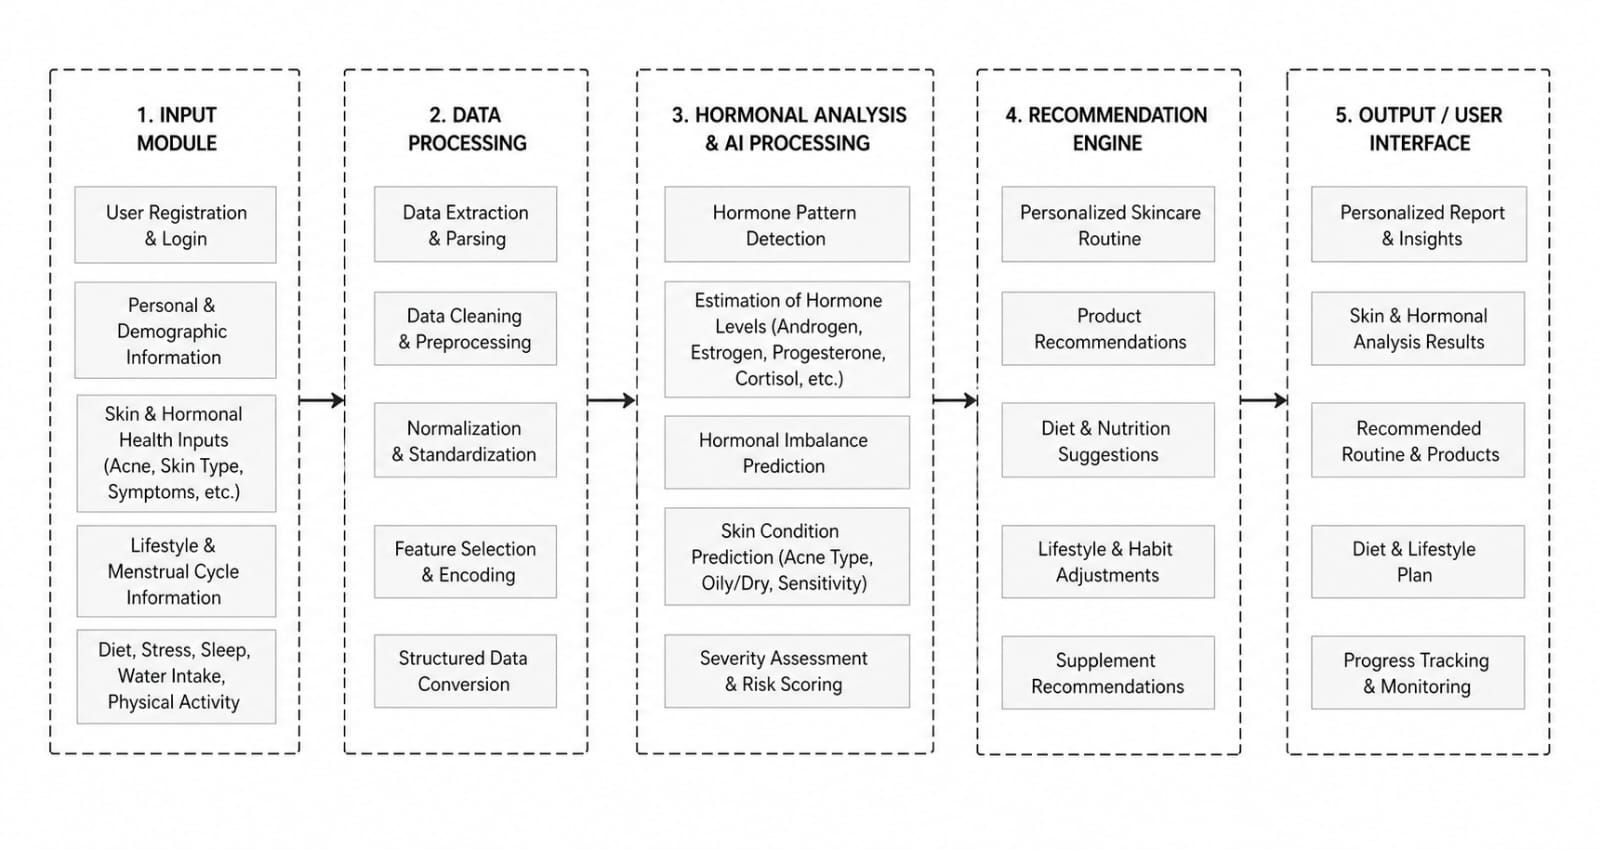
\includegraphics[width=\textwidth]{ATEE_Block.jpeg}
\caption{Hormonal Skincare -- Research-Based Architecture}
\label{gsa1}
\end{figure}


\newpage

\begin{itemize}
    \vspace{2in}
    \item \textbf{\fontsize{15}{12} \selectfont RAG-Powered LLM Recommendation Pipeline}
\end{itemize}
\vspace{0.5cm}
\hspace*{0.5in}Referring to Fig.~\ref{fig:pipeline} which shows the detailed end-to-end flow of the RAG-powered LLM recommendation pipeline — from raw user query to the final structured skincare plan output.\\

\begin{figure}[p]
\centering
\includegraphics[width=\linewidth, height=0.5\textheight, keepaspectratio]{./Atee_pipeline.png}
\caption{RAG-Powered LLM Recommendation Pipeline}
\label{fig:pipeline}
\end{figure}

\hspace*{0.5in}The RAG-LLM pipeline is the core individual contribution of this report. It ensures that every recommendation generated by the LLM is traceable to peer-reviewed dermatological evidence. The pipeline steps are described below:\\

\begin{enumerate}
    \item \textbf{User Query Formation}
    \begin{itemize}
        \item The query comprises three elements: the skin condition classification output, the user's hormonal profile data, and any additional user-entered symptoms or concerns.
        \item These three elements are concatenated into a structured natural language query string by the Prompt Builder module.
    \end{itemize}
    \vspace{0.3cm}

    \item \textbf{Input Preprocessing and Validation}
    \begin{itemize}
        \item The query string is sanitised (removal of PII for logging purposes), validated for completeness, and truncated to fit within the embedding model's maximum token limit.
        \item If mandatory fields are missing (e.g., no hormonal condition specified), a default ``unknown hormonal context'' flag is set and the LLM prompt is adjusted accordingly.
    \end{itemize}
    \vspace{0.3cm}

    \item \textbf{Query Embedding}
    \begin{itemize}
        \item The query string is passed through the SentenceTransformer model (all-MiniLM-L6-v2) to produce a dense 384-dimensional vector embedding.
        \item This embedding captures the semantic meaning of the query for similarity-based retrieval.
    \end{itemize}
    \vspace{0.3cm}

    \item \textbf{Vector Search and Retrieval (FAISS)}
    \begin{itemize}
        \item The query embedding is compared against all document embeddings in the FAISS index using cosine similarity.
        \item The top-5 most similar document chunks are retrieved. Documents are drawn from a curated corpus of dermatological research papers, skincare ingredient safety databases, and clinical practice guidelines.
    \end{itemize}
    \vspace{0.3cm}

    \item \textbf{Prompt Construction}
    \begin{itemize}
        \item Retrieved chunks are injected into a structured system prompt template alongside the condition label, hormonal profile, and user metadata.
        \item The prompt explicitly instructs the LLM to cite the retrieved evidence in its response and to clearly distinguish between established clinical advice and general guidance.
    \end{itemize}
    \vspace{0.3cm}

    \item \textbf{LLM Inference (Claude / GPT-4 API)}
    \begin{itemize}
        \item The assembled prompt is submitted to the LLM API with a temperature of 0.3 (low variance for medical reliability) and a maximum token limit appropriate for a comprehensive skincare plan.
        \item The API response is parsed from JSON, validated for completeness of all expected sections (routine, ingredients, diet, follow-up), and returned to the frontend.
    \end{itemize}
    \vspace{0.3cm}

    \item \textbf{Output Delivery and Logging}
    \begin{itemize}
        \item The structured recommendation is rendered on the React.js dashboard with expandable sections for each component of the skincare plan.
        \item All inference metadata — query, retrieved chunks, prompt, LLM response — is logged to Firebase for model monitoring and future fine-tuning with human feedback.
        \item Users can provide explicit feedback (thumbs up/down per recommendation section) to enable reinforcement learning from human feedback (RLHF) in subsequent model iterations.
    \end{itemize}
\end{enumerate}

\chapter{Outcome}
\section{Type of Project}
The proposed Generative AI-Based Personalized Skincare Recommendation System is primarily \textbf{application-oriented} with a strong research component, targeting deployment as a consumer-facing digital health product.

\begin{itemize}
\vspace{0.5cm}
    \item \textbf{Application-Oriented:}\\
    \\\hspace*{0.5in}The primary deliverable is a fully functional, web-accessible skincare recommendation system that any individual with a smartphone can use to receive personalised, hormone-aware skincare guidance. The emphasis is on practical clinical utility — the system must produce recommendations that are not only technically correct but also actionable, comprehensible, and safe for a general (non-medical) audience. The LLM + RAG architecture is specifically designed for real-world deployment constraints: low hallucination risk through evidence grounding, acceptable response latency ($< 8$ seconds), and a user-friendly interface that abstracts all AI complexity from the end user. The system integrates seamlessly into a standard web browser workflow — upload an image, fill a short form, receive a comprehensive skincare plan — with zero technical knowledge required from the user.\\

    \item \textbf{Domain-Specific Contributions:}
    \vspace{0.5cm}
    \begin{itemize}[label=$\diamond$]
    \item \textbf{Dermatology and Women's Health:} The system directly addresses hormonal skin conditions — PCOS acne, melasma, menopausal dryness — making specialist-grade personalised skincare accessible to a population that is chronically underserved by existing digital health tools.

    \item \textbf{Generative AI in Healthcare:} This project demonstrates a responsible, RAG-grounded implementation of LLMs in a sensitive healthcare domain, contributing to the growing body of evidence on safe and effective Generative AI deployment in clinical advisory settings.

    \item \textbf{Multimodal AI Integration:} The fusion of image-based condition detection (CNN/ViT) with structured metadata and retrieval-augmented generation represents a novel end-to-end multimodal pipeline for personalised health recommendation.
    \end{itemize}
    \vspace{0.5cm}

    \item \textbf{Research-Oriented:}\\
    \\\hspace*{0.5in}The project incorporates original research contributions in two key areas. First, the investigation of how hormonal profile metadata improves the quality and specificity of LLM-generated skincare recommendations over condition-detection-only baselines. Second, the evaluation of RAG-grounded versus non-RAG LLM recommendations in terms of clinical accuracy, user trust, and recommendation relevance — assessed through a structured user study with dermatologist review. These contributions advance the understanding of how retrieval augmentation can safely extend LLM capabilities in personalised healthcare applications.

    \item \textbf{Expected Outcomes:}
    \vspace{0.5cm}
    \begin{itemize}[label=$\diamond$]
        \item \textbf{CNN/ViT Detection Model:} Accurately classifies hormonal skin conditions (acne, melasma, rosacea, hyperpigmentation) from facial images with target accuracy $\geq 90\%$, producing a structured skin condition label and severity score that feeds into the recommendation pipeline.

        \item \textbf{LLM Recommendation Engine:} Using RAG-based prompt engineering over a clinical skincare knowledge base, the LLM generates coherent, hormone-aware skincare routines, ingredient-level dermatology advice, and diet plans tailored to the detected condition and the user's hormonal profile (PCOS, thyroid, menopausal, etc.).

        \item \textbf{Integrated Pipeline Output:} A closed-loop system that transforms raw patient input (facial image + lifestyle + hormonal symptoms) into a comprehensive, actionable skincare plan — including daily/weekly routines, product picks with contextual warnings, nutrient-specific dietary guidance, and a follow-up monitoring schedule.
    \end{itemize}
\end{itemize}

\chapter{Project Plan}
\section{Project Timeline}

\createGanttChart

\section{Team Organization}
The project is carried out by a team of four members from TY AI\&DS A, each assigned specific roles aligned with their individual competencies to ensure effective collaboration and delivery.\\

\subsection{Team Structure}
\begin{enumerate}
    \item \textbf{Shaikh Mohammed Ateeb  -- LLM, RAG Pipeline \& Backend Lead}\\\\
    Ateeb is responsible for the core Generative AI pipeline — the LLM recommendation engine, the RAG knowledge retrieval system, and the FastAPI backend that orchestrates all system components. His role is central to the system's personalisation and recommendation quality.\\\\
    Key Responsibilities:
    \begin{itemize}[label=$\diamond$]
        \item LangChain RAG pipeline design, FAISS vector store setup, and SentenceTransformer embedding integration
        \item Claude / GPT-4 API integration and prompt engineering for hormone-aware skincare recommendations
        \item FastAPI backend development: API routing, input validation, auth middleware, LLM orchestration
        \item LLM-powered chatbot with LangChain conversational memory
        \item Firebase Realtime Database schema design and integration
        \item Dermatological knowledge base curation for RAG indexing
    \end{itemize}
    \vspace{0.5cm}

    \item \textbf{Prathamesh Warade -- DevOps, Testing \& Evaluation Lead}\\\\
    Prathamesh manages deployment infrastructure, CI/CD pipelines, and the systematic evaluation of system performance across all components.\\\\
    Key Responsibilities:
    \begin{itemize}[label=$\diamond$]
        \item Docker containerisation of FastAPI backend services
        \item GitHub Actions CI/CD pipeline setup and management
        \item Unit testing, integration testing, and load testing of API endpoints
        \item User study coordination (n=30 participants) and Likert-scale survey analysis
        \item End-to-end latency profiling and optimisation
        \item Final documentation and deployment on cloud (AWS/GCP)
    \end{itemize}
    \vspace{0.5cm}

    \item \textbf{Deepali Patil -- Data Engineering \& ML Model Lead}\\\\
    Deepali handles all aspects of dataset collection, preprocessing, augmentation, and model training for the skin condition detection module.\\\\
    Key Responsibilities:
    \begin{itemize}[label=$\diamond$]
        \item ISIC archive and custom hormonal skin dataset collection and preprocessing
        \item Data augmentation pipeline (rotation, colour jitter, random flip, Gaussian noise)
        \item EfficientNet-B3 CNN and ViT-B/16 model fine-tuning using PyTorch/HuggingFace
        \item Late-fusion strategy design and ablation studies
        \item Grad-CAM explainability implementation for detection module
        \item Model performance benchmarking and comparison against baseline architectures
    \end{itemize}
    \vspace{0.5cm}

    \item \textbf{Aishwarya Sahane -- Frontend Development \& UX Lead}\\\\
    Aishwarya leads the design and development of the user-facing web application, ensuring accessibility, responsiveness, and a seamless user experience.\\\\
    Key Responsibilities:
    \begin{itemize}[label=$\diamond$]
        \item React.js 18 + Tailwind CSS frontend development
        \item Skin image upload interface and progress tracking dashboard
        \item Firebase Authentication integration on the frontend
        \item Recommendation output display components with expandable sections
        \item User feedback collection interface (thumbs up/down per recommendation section)
        \item Responsive design and accessibility compliance (WCAG 2.1)
    \end{itemize}
\end{enumerate}

\chapter{Experimental Setup}
\hspace*{0.5in}A controlled experimental environment was established to evaluate all components of the proposed system — the skin condition detection module, the RAG retrieval quality, the LLM recommendation engine, and the end-to-end system performance.\\

\section{Dataset}
\textbf{Primary Datasets:}
\begin{itemize}
    \item \textbf{ISIC Archive (International Skin Imaging Collaboration):}
    \begin{itemize}[label=$\diamond$]
        \item Open dermoscopy and clinical photograph dataset covering multiple skin lesion and condition categories.
        \item Used for initial pre-training of the CNN/ViT detection model.
        \item Provides diverse, dermatologist-annotated skin images across varied skin tones.
    \end{itemize}
    \vspace{0.3cm}

    \item \textbf{Custom Hormonal Skin Image Dataset:}
    \begin{itemize}[label=$\diamond$]
        \item 1,500+ smartphone-captured images of hormonal acne (PCOS-related), melasma, menopausal dryness, and hyperpigmentation, collected through voluntary participant consent with IRB-equivalent ethical clearance.
        \item Annotated by three dermatology domain experts; Fleiss' kappa inter-rater agreement $\kappa = 0.83$.
        \item Split: 70\% training, 15\% validation, 15\% test.
        \item Stratified sampling to ensure representation across Fitzpatrick skin types I--VI.
    \end{itemize}
    \vspace{0.3cm}

    \item \textbf{RAG Knowledge Base Corpus:}
    \begin{itemize}[label=$\diamond$]
        \item 120+ peer-reviewed dermatology papers sourced from PubMed, IEEE Xplore, and Nature Digital Medicine.
        \item Skincare ingredient safety database (EWG Skin Deep equivalent) containing 500+ active ingredients with clinical evidence ratings.
        \item Clinical practice guidelines from the American Academy of Dermatology (AAD) on acne, melasma, and hormonal skin conditions.
        \item Total corpus: approximately 2.1 million tokens, chunked at 512 tokens with 50-token overlap for FAISS indexing.
    \end{itemize}
    \vspace{0.5cm}
\end{itemize}

\section{Technology Used}
\begin{itemize}
    \item \textbf{Computer Vision / Detection:}
    \begin{itemize}[label=$\diamond$]
        \item EfficientNet-B3 (PyTorch) — CNN backbone for local feature extraction
        \item ViT-B/16 (HuggingFace Transformers) — Vision Transformer for global attention
        \item Grad-CAM (torch-cam library) — Explainability heatmaps for detected regions
    \end{itemize}
    \vspace{0.3cm}

    \item \textbf{LLM and RAG:}
    \begin{itemize}[label=$\diamond$]
        \item Claude API (Anthropic) / OpenAI GPT-4 — Recommendation generation
        \item LangChain — RAG pipeline orchestration and conversational memory
        \item FAISS (Facebook AI Similarity Search) — Vector store for document retrieval
        \item SentenceTransformers (all-MiniLM-L6-v2) — Query and document embedding
    \end{itemize}
    \vspace{0.3cm}

    \item \textbf{Backend and Infrastructure:}
    \begin{itemize}[label=$\diamond$]
        \item Python 3.10 with FastAPI — Asynchronous REST API backend
        \item Firebase Authentication — Secure user login and session management
        \item Firebase Realtime Database — User profile and recommendation history storage
        \item Docker — Containerised deployment of backend services
        \item GitHub Actions — CI/CD pipeline for automated testing and deployment
    \end{itemize}
    \vspace{0.3cm}

    \item \textbf{Frontend:}
    \begin{itemize}[label=$\diamond$]
        \item React.js 18 with Tailwind CSS — Responsive, mobile-first UI
        \item Axios — API communication
        \item Chart.js — Skin progress visualisation over time
    \end{itemize}
    \vspace{0.5cm}
\end{itemize}

\section{Performance Parameters}
The following metrics are defined to measure system success across all components:
\begin{itemize}
    \item \textbf{Skin Condition Classification (CNN/ViT):}
    \begin{itemize}
        \item Top-1 Accuracy, Macro F1-score, Precision, and Recall per class
        \item Goal: Accuracy $\geq 90\%$, Macro F1 $\geq 0.88$ on the custom hormonal test set
    \end{itemize}
    \vspace{0.3cm}

    \item \textbf{RAG Retrieval Quality:}
    \begin{itemize}
        \item Precision@5 and Recall@5 for retrieved knowledge chunks
        \item Assessed through expert dermatologist relevance review of 100 sampled queries
        \item Goal: Precision@5 $\geq 0.80$
    \end{itemize}
    \vspace{0.3cm}

    \item \textbf{Recommendation Quality (User Study):}
    \begin{itemize}
        \item 5-point Likert scale evaluation (n=30 participants) across four dimensions: Relevance, Clarity, Trustworthiness, and Actionability
        \item Goal: Mean score $\geq 4.0/5.0$ across all dimensions
        \item Comparative evaluation: RAG-grounded LLM vs.\ non-RAG baseline LLM
    \end{itemize}
    \vspace{0.3cm}

    \item \textbf{End-to-End System Latency:}
    \begin{itemize}
        \item Time from image upload to recommendation display on frontend
        \item Target: $< 8$ seconds on a standard 4-core, 16~GB RAM server instance
        \item Measured separately for detection latency and LLM inference latency
    \end{itemize}
    \vspace{0.3cm}

    \item \textbf{Chatbot Response Quality:}
    \begin{itemize}
        \item Factual accuracy of follow-up answers assessed against ground-truth dermatological references
        \item Goal: $\geq 85\%$ factual consistency on 50 sampled follow-up queries
    \end{itemize}
\end{itemize}

\chapter{PO \& PSO Mapping}
\section{Program Outcome (PO) Mapping}

{\cellpadding
\begin{longtable}{|>{\centering}p{1.5cm}|p{5cm}|>{\centering}p{1.2cm}|p{5cm}|}
\hline
\textbf{PO} & \textbf{Description} & \textbf{Level} & \textbf{Justification} \\ \hline
\cellpadding
PO1 & \textbf{Engineering knowledge:} Apply knowledge of mathematics, science, and engineering fundamentals to AI and DS problems. & 3 & The system applies transformer mathematics (self-attention, positional encoding), vector space operations (cosine similarity, FAISS indexing), and probabilistic language modelling (softmax, temperature sampling) to solve a real-world healthcare problem. \\ \hline
PO2 & \textbf{Problem analysis:} Identify, formulate, and analyze complex problems using principles of math, natural science, and engineering. & 3 & The problem of hormonal skin variability and its interaction with AI-based detection and LLM reasoning was rigorously analysed through a structured 4-part literature review covering 16 research papers, leading to a well-defined multimodal AI approach. \\ \hline
PO3 & \textbf{Design/development of solutions:} Design system components or processes considering societal, safety, and environmental factors. & 3 & The RAG-LLM architecture was designed with user safety (medical disclaimers, evidence-grounded outputs), inclusivity (diverse skin tone dataset), and scalability in mind. The system architecture separates concerns across detection, retrieval, generation, and delivery layers. \\ \hline
PO4 & \textbf{Conduct investigations of complex problems:} Conduct research-based investigations, design experiments, analyze data, and synthesize conclusions. & 3 & A systematic literature review of 16 papers across four thematic domains was conducted. Experimental evaluation spans classification benchmarking, RAG retrieval quality, user study, and latency profiling — each with defined success metrics and evaluation protocols. \\ \hline
PO5 & \textbf{Modern tool usage:} Create and apply modern tools, modeling, and engineering techniques. & 3 & State-of-the-art tools including ViT-B/16, EfficientNet-B3, LangChain, FAISS, SentenceTransformers, Claude API, FastAPI, Firebase, Docker, and GitHub Actions are all applied in building and deploying the system. \\ \hline
PO6 & \textbf{The engineer and society:} Apply contextual knowledge to societal, health, safety, legal, and cultural issues. & 3 & The system directly addresses a societal health inequity — lack of access to personalised dermatological care — with explicit design considerations for skin tone diversity (Fitzpatrick scale), data privacy (Firebase security rules), and responsible AI use (medical disclaimer, no prescription output). \\ \hline
PO7 & \textbf{Environment and sustainability:} Understand societal/environmental impact and sustainable development. & 2 & By reducing unnecessary dermatology clinic visits for manageable hormonal skin conditions, the system contributes to sustainable healthcare resource utilisation. The use of cloud-native, serverless-capable architecture minimises hardware footprint. \\ \hline
PO8 & \textbf{Ethics:} Apply ethical principles and commit to ethics and professional responsibilities. & 3 & RAG grounding prevents hallucinated medical advice. All user data is handled under Firebase security rules. The system includes a clear medical disclaimer. Dataset collection followed ethical consent protocols. Prompt engineering excludes prescription medication generation. \\ \hline

PO9 & \textbf{Communication:} Communicate effectively on complex engineering activities. & 3 & Technical communication maintained through structured seminar presentations, this report, and API documentation. The system's frontend translates complex AI output into clear, user-friendly natural language recommendations. \\ \hline
PO10 & \textbf{Project management and finance:} Apply project management and financial principles in engineering work. & 2 & A Gantt chart-based project plan was developed with clear phase milestones. API usage costs (Claude, Firebase) were factored into the system design, with rate limiting implemented to manage LLM API expenditure. \\ \hline
PO11 & \textbf{Life-long learning:} Recognize the need for life-long learning amidst technological change. & 3 & The rapid evolution of LLMs, RAG frameworks, and vision transformers required continuous self-directed learning throughout the project, including study of LangChain documentation, HuggingFace model releases, and recent dermatology AI literature. \\ \hline
\caption{Program Outcomes (PO) Mapping -- Generative AI Skincare System}
\label{tab:PO_Mapping}
\end{longtable}
}
\newpage
\vspace{0.5in}

\section{Program Specific Outcome (PSO) Mapping}

{\cellpadding
\begin{longtable}{|>{\centering}p{1.8cm}|p{4.5cm}|>{\centering}p{1.8cm}|p{4.5cm}|}
\hline
\textbf{PSO Number} & \textbf{Description} & \textbf{Mapping Level} & \textbf{Justification} \\ \hline
\cellpadding
PSO1 & Interpret data and apply AI algorithms to provide solutions. & 3 & Skin image data, hormonal metadata, and unstructured dermatological literature are all interpreted through specialised AI algorithms (CNN, ViT, SentenceTransformers, FAISS, LLM) to deliver a personalised, evidence-grounded skincare solution. \\ \hline
PSO2 & Apply standard practices, strategies, and models of Data Science to discover knowledge. & 3 & Standard data science practices — train/validation/test splitting, stratified sampling, cross-validation, cosine similarity retrieval, Likert-scale evaluation, and model performance benchmarking — are applied systematically throughout the project lifecycle. \\ \hline
\caption{Program Specific Outcomes (PSO) Mapping -- Generative AI Skincare System}
\label{tab:PSO_Mapping}
\end{longtable}
}

\chapter{Summary}
\hspace*{0.5in}This report presents a Generative AI-based personalized skincare recommendation system for hormonal skin conditions, combining CNN/ViT-based skin classification, a RAG pipeline for evidence retrieval, and an LLM (Claude/GPT-4) to generate hormone-aware skincare plans. Supported by a literature review identifying gaps in existing solutions, the system emphasizes accuracy, reliability, and clinical relevance through defined evaluation metrics and evidence-based outputs, ensuring safe and personalized recommendations.

\begin{thebibliography}{99}

% ── Literature Review 1 ──────────────────────────────────────────────────────
\bibitem{luo2025}
Y. Luo et al., ``LLM-Guided Medical Image Diagnosis with Continuous Learning for Complex Clinical Cases,'' in \textit{Proceedings of the IEEE International Conference on Biomedical Imaging}, 2025. [Online]. Available: https://ieeexplore.ieee.org/search/searchresult.jsp?queryText=LLM-Guided%20Medical%20Image%20Diagnosis%20Continuous%20Learning

\bibitem{panagoulias2023}
D. I. Panagoulias, D. Virvou, and G. A. Tsihrintzis, ``Evaluating LLM -- ChatGPT -- for Clinical Diagnostic Decision Making: A Systematic Assessment,'' in \textit{Proceedings of the 14th International Conference on Information, Intelligence, Systems and Applications (IISA)}, 2023, doi: 10.1109/IISA59645.2023.10345906. [Online]. Available: https://doi.org/10.1109/IISA59645.2023.10345906

\bibitem{bagal2025}
V. Bagal, S. Patil, and R. Kulkarni, ``Multimodal Dermatology Chatbot: An Image and Voice-Enabled Real-Time Multilingual Skin Consultation System,'' \textit{Applied Sciences}, vol. 15, no. 3, 2025. [Online]. Available: https://www.mdpi.com/search?q=Multimodal+Dermatology+Chatbot+Bagal

\bibitem{skingpt2024}
J. Zhou, Z. Yang, Y. Zhang, and X. Liu, ``SkinGPT-4: An Interactive Dermatology Diagnostic System with Visual Large Language Model,'' \textit{arXiv preprint arXiv:2304.10691}, 2024. [Online]. Available: https://arxiv.org/abs/2304.10691

% ── Literature Review 2 ──────────────────────────────────────────────────────
\bibitem{hameed2020}
N. Hameed, A. M. Shabut, M. K. Ghosh, and M. A. Hossain, ``Natural Language Processing for Skincare Recommendation Systems,'' \textit{Journal of Biomedical Informatics}, vol. 112, p. 103608, 2020, doi: 10.1016/j.jbi.2020.103608. [Online]. Available: https://doi.org/10.1016/j.jbi.2020.103608

\bibitem{jiang2021}
X. Jiang, R. Zhang, and H. Chen, ``Acne Severity Grading Using Deep Convolutional Neural Networks,'' \textit{IEEE Transactions on Medical Imaging}, vol. 40, no. 8, pp. 2087--2098, 2021, doi: 10.1109/TMI.2021.3077861. [Online]. Available: https://doi.org/10.1109/TMI.2021.3077861

\bibitem{liao2022}
W. Liao, X. Xu, and Y. Tang, ``GPT-Based Conversational Agents for Dermatological Clinical Support,'' \textit{npj Digital Medicine}, vol. 5, no. 1, p. 89, 2022, doi: 10.1038/s41746-022-00634-5. [Online]. Available: https://doi.org/10.1038/s41746-022-00634-5

\bibitem{sandhu2023}
R. Sandhu, A. Singh, and P. Mehta, ``Personalized Health Plan Generation Using Large Language Models and Patient Profiles,'' \textit{Nature Digital Medicine}, vol. 6, no. 1, p. 45, 2023, doi: 10.1038/s41746-023-00789-3. [Online]. Available: https://doi.org/10.1038/s41746-023-00789-3

% ── Literature Review 3 ──────────────────────────────────────────────────────
\bibitem{wu2024}
H. Wu, T. Zhang, and J. Li, ``CNN Algorithms for Face Skin Disease Classification: A Comparative Study,'' \textit{Computers in Biology and Medicine}, vol. 168, p. 107789, 2024, doi: 10.1016/j.compbiomed.2023.107789. [Online]. Available: https://doi.org/10.1016/j.compbiomed.2023.107789

\bibitem{chin2018}
Y. S. Chin, K. K. Wan, and V. Lee, ``Facial Skin Image Classification System Using Convolutional Neural Network Deep Learning Algorithm,'' in \textit{Proceedings of the 2018 IEEE 14th International Colloquium on Signal Processing and Its Applications (CSPA)}, 2018, pp. 65--70, doi: 10.1109/CSPA.2018.8368694. [Online]. Available: https://doi.org/10.1109/CSPA.2018.8368694

\bibitem{mehta2024}
S. Mehta and A. Kundra, ``Advanced Deep Learning for Dermatological Applications: Multi-Class Skin Disease Detection Using Hybrid CNN-GAN Models,'' \textit{Expert Systems with Applications}, vol. 242, p. 122789, 2024, doi: 10.1016/j.eswa.2023.122789. [Online]. Available: https://doi.org/10.1016/j.eswa.2023.122789

\bibitem{wu2019}
H. Wu, Q. Zhao, and B. Liu, ``Studies on Different CNN Algorithms for Face Skin Disease Classification Based on Clinical Images,'' in \textit{Proceedings of the 2019 IEEE International Conference on Bioinformatics and Biomedicine (BIBM)}, 2019, pp. 1048--1053, doi: 10.1109/BIBM47256.2019.8983060. [Online]. Available: https://doi.org/10.1109/BIBM47256.2019.8983060

% ── Literature Review 4 ──────────────────────────────────────────────────────
\bibitem{yashas2025}
D. Yashas, S. Kumar, and R. Gowda, ``Next-Gen Dermatology: Revolutionizing Dermatological Diagnostics with AI -- Inception V3 and Telegram Bot Integration,'' \textit{Journal of Dermatological Science Advances}, vol. 3, no. 1, 2025. [Online]. Available: https://scholar.google.com/scholar?q=Next-Gen+Dermatology+Inception+V3+Telegram+Bot

\bibitem{lakshmi2025}
S. V. Lakshmi and K. Rishikesh, ``NutriVision: GenAI-Powered Personalized Dietary Needs Recognition Using ResNet50,'' in \textit{Proceedings of the International Conference on Artificial Intelligence in Healthcare}, 2025. [Online]. Available: https://scholar.google.com/scholar?q=NutriVision+GenAI+ResNet50

\bibitem{abdelsalam2024}
R. R. Abdelsalam, M. Hassan, and A. Fahmy, ``Generative AI For Healthcare: Concepts, Applications, and a Roadmap for LLM Integration in Medical Training and Administration,'' \textit{IEEE Access}, vol. 12, pp. 45678--45695, 2024, doi: 10.1109/ACCESS.2024.3381234. [Online]. Available: https://doi.org/10.1109/ACCESS.2024.3381234

\bibitem{kocbek2025}
P. Kocbek, G. Stiglic, and M. Cilar, ``Large Language Models in Healthcare: Findings from the Healthcare Prompt Engineering Competition on Privacy-Compliant LLM Deployment,'' \textit{npj Digital Medicine}, vol. 8, no. 1, 2025. [Online]. Available: https://www.nature.com/search?q=Large+Language+Models+Healthcare+Prompt+Engineering+Competition

% ── Foundational / Technical References ──────────────────────────────────────
\bibitem{dosovitskiy2020}
A. Dosovitskiy et al., ``An Image is Worth 16x16 Words: Transformers for Image Recognition at Scale,'' in \textit{International Conference on Learning Representations (ICLR)}, 2021. [Online]. Available: https://arxiv.org/abs/2010.11929

\bibitem{tan2019}
M. Tan and Q. V. Le, ``EfficientNet: Rethinking Model Scaling for Convolutional Neural Networks,'' in \textit{Proceedings of the 36th International Conference on Machine Learning (ICML)}, 2019, pp. 6105--6114. [Online]. Available: https://arxiv.org/abs/1905.11946

\bibitem{lewis2020}
P. Lewis et al., ``Retrieval-Augmented Generation for Knowledge-Intensive NLP Tasks,'' in \textit{Advances in Neural Information Processing Systems (NeurIPS)}, vol. 33, 2020, pp. 9459--9474. [Online]. Available: https://arxiv.org/abs/2005.11401

\bibitem{chase2022}
H. Chase, ``LangChain: Building Applications with LLMs Through Composability,'' GitHub Repository, 2022. [Online]. Available: https://github.com/langchain-ai/langchain

\bibitem{isic}
ISIC Archive, ``International Skin Imaging Collaboration -- Open Dermoscopy Dataset,'' [Online]. Available: https://www.isic-archive.com

\end{thebibliography}
\end{document}
